% Generated from ../engineering-argumentation-ai-agents.md by reproduction/typeset.py.
% Edit the maintained prose there; regenerate this complete, editable LaTeX source.
\documentclass[11pt,a4paper]{article}
\usepackage[T1]{fontenc}
\usepackage[utf8]{inputenc}
\usepackage{lmodern,microtype}
\usepackage[a4paper,textwidth=155mm,top=24mm,bottom=24mm]{geometry}
\usepackage{amsmath,amssymb,booktabs,longtable,array,calc}
\usepackage{graphicx,xcolor,tikz,pgfplots}
\pgfplotsset{compat=1.18}
\usepackage{xurl,caption,placeins,flafter,needspace}
\usepackage[colorlinks=true,linkcolor=black,citecolor=black,urlcolor=teal!65!black]{hyperref}
\hypersetup{pdftitle={Engineering argumentation with AI agents},pdfsubject={Explicit justification and minimum sufficient evidence for engineering decisions}}
\captionsetup{font=small,labelfont=bf,skip=8pt}
\setlength{\parindent}{0pt}
\setlength{\parskip}{5.5pt plus 1pt minus 1pt}
\setlength{\emergencystretch}{2em}
\setlength{\LTpre}{8pt}
\setlength{\LTpost}{8pt}
\setlength{\tabcolsep}{5pt}
\renewcommand{\arraystretch}{1.12}
\clubpenalty=10000
\widowpenalty=10000
\displaywidowpenalty=10000
\postdisplaypenalty=10000
\raggedbottom
\begin{document}
{\fontsize{22}{26}\selectfont\bfseries Engineering argumentation\\with AI agents\par}
\vspace{4pt}
{\large Justification and minimum sufficient evidence\par}
\vspace{5pt}
{\small 3 October 2026\par}
\vspace{10pt}
\textbf{Consequential delegation to AI agents requires explicit, challengeable justification. Engineers should construct that justification by thinking through the decision and obtaining the minimum sufficient evidence for the resulting action.} Increasing the volume of assurance work or the number of approvals does not by itself improve either judgement or outcomes. The proposed change in practice is to make the reasons for consequential delegation inspectable, proportionate and revisable throughout use.

An engineering argument explains why particular grounds support a particular conclusion, under stated conditions, and how contrary evidence could alter it. Its purpose here is to justify a decision or reliance on a claim. Argumentation includes constructing, challenging and revising that account. It can be expressed in a short review comment, a calculation with explicit assumptions, a decision record or an executable representation. Length and notation are secondary to the adequacy of the reasoning.

The proposition that traditional engineering excluded argumentation is historically untenable. NASA's systems-engineering guidance already calls for documented decision rationale, alternatives, assumptions and uncertainty. The Software Engineering Institute described evidence-supported safety arguments for medical devices in 2009. The assurance-case standard ISO/IEC/IEEE 15026-2 has a 2011 predecessor. These establish a pre-existing engineering practice; they do not establish how consistently every organisation applied it.\cite{nasa,sei,standard}

The defensible thesis therefore concerns a change in the \textbf{default use and maintenance of explicit justification} wherever AI receives consequential engineering responsibilities. In organisations already maintaining adequate assurance arguments, this is an extension of established practice. In organisations whose reasoning remains dispersed across conversations, artefacts and individual memory, it would change what must accompany an accepted result. Calling this a paradigm shift is a proposal about engineering practice, rather than an established finding that the whole profession has already changed.

Established engineering methods continue to supply the evidence and controls on which that justification depends. The following comparison uses NASA's verification, validation and technical-management processes as one documented baseline; the final column is the engineering recommendation developed here.\cite{nasa}

\begin{table}[htbp]
\small
\centering
\caption[Established engineering practices]{Established engineering practices and their contribution to AI-assisted decisions.}\label{tab:practices}
\begin{tabular}{@{}
  >{\raggedright\arraybackslash}p{(\columnwidth - 4\tabcolsep) * \real{0.26}}
  >{\raggedright\arraybackslash}p{(\columnwidth - 4\tabcolsep) * \real{0.29}}
  >{\raggedright\arraybackslash}p{(\columnwidth - 4\tabcolsep) * \real{0.45}}@{}}
\toprule\noalign{}
\begin{minipage}[b]{\linewidth}\raggedright
Established practice
\end{minipage} & \begin{minipage}[b]{\linewidth}\raggedright
Continuing function
\end{minipage} & \begin{minipage}[b]{\linewidth}\raggedright
Question the argument must answer when AI contributes
\end{minipage} \\[4pt]
\midrule\noalign{}
Requirements and acceptance criteria & Define the intended result and constraints & Does the criterion express the stakeholder's actual need, and who established it? \\[4pt]
Calculation, modelling and formal analysis & Derive consequences from an explicit model & Do the model, premises and operating conditions apply to this decision? \\[4pt]
Testing, inspection and verification & Check specified properties of an identified artefact & What does this result establish, and which relevant failures could the method miss? \\[4pt]
Validation and operational trials & Assess suitability for intended use & Does the observed behaviour transfer to the proposed environment and users? \\[4pt]
Technical review and risk analysis & Challenge design choices and examine adverse consequences & Which objection could change the choice, and has it been answered? \\[4pt]
Configuration control and operational monitoring & Identify the accepted state and detect relevant changes & Which earlier conclusions remain applicable after this change? \\[4pt]
\bottomrule
\end{tabular}
\end{table}

AI adoption provides a reason to address these questions now, although adoption figures need careful interpretation. The US Census Bureau reported AI use by 19.8\% of businesses in the collection period ending 3 May 2026; its question concerns any business function and was broadened in November 2025. This is not an autonomous-agent prevalence estimate.\cite{census} Microsoft's 2025 survey reported that 46\% of surveyed leaders said their companies used agents to automate workflows or processes. The underlying survey covered 31,000 knowledge workers across 31 markets. This vendor-sponsored, self-reported sample does not establish that 46\% of all organisations deploy autonomous agents.\cite{microsoft} The argument below applies to consequential deployments whether their economy-wide prevalence is high or low.

An AI agent, for this discussion, is a software system that uses a model to select and sequence tool-mediated actions towards a task objective. The relevant change is the scope of delegated activity. An agent may help formulate a requirement, implement a change, select its tests and explain its apparent success. If these steps share a mistaken interpretation, the resulting artefacts can agree while failing the intended requirement. This is an engineering failure mechanism, not an estimate of its frequency. Independently checking an outcome against a separately established criterion addresses that mechanism more directly than obtaining another agreeable explanation from the same process.

Empirical research establishes reasons to investigate this mechanism without supporting a universal claim that AI worsens engineering. Perry and colleagues' 47-participant study found security disadvantages and greater confidence in code security with an older AI assistant on selected programming tasks. Its sample, tasks and model restrict generalisation.\cite{perry} Sandoval and colleagues' separate 58-participant C-programming study found a small security impact in its setting, challenging a blanket adverse conclusion.\cite{sandoval} In a different workplace, Brynjolfsson and colleagues studied a staggered rollout to 5,172 customer-support workers and estimated a 15\% average productivity increase, with heterogeneous effects. Those support agents were people receiving AI assistance.\cite{benefits} The defensible inference is that the actual task, model and workflow need assessment; favourable or adverse results from another setting cannot decide the present case.

Tool use also exposes a distinction between information and authority. AgentDojo evaluated 97 tasks and 629 security test cases involving agents and untrusted tool content. Its experiments demonstrate that prompt injection can violate some security properties and that task failures can also occur without attacks. They provide benchmark evidence of possible failure, rather than workplace incident rates.\cite{agentdojo} NIST's Generative AI Profile identifies confabulation and problematic human reliance, and recommends context-sensitive evaluation and verification of sources.\cite{genai} These findings support externally checkable evidence and enforced action boundaries. A persuasive argument supplied by an agent cannot grant the agent permission to act.

The warrant connecting these observations to the first claim is an engineering requirement for justified reliance: \textbf{when accepting a consequential result requires an inference beyond what a test, proof or observation directly establishes, the responsible engineer must assess why that inference applies}. A passing test establishes a result for its inputs, oracle and configuration. Extending it to a deployment requires a defensible account of coverage and applicability. A formal proof similarly depends on the specification, model and correspondence with the implemented system. Where an existing review or assurance process already provides that account, the requirement is met there. Where it does not, adding more passing results leaves the missing inference unresolved.

The necessity claimed is conditional and practical. It concerns making decision-relevant reasoning available for scrutiny when work passes between people, agents or sessions. It does not establish that every small task requires a separate argument document, that Toulmin is the only suitable method, or that EAL is required. A fully checked bounded decision procedure can discharge routine cases under an already justified rule; engineers then examine exceptions and changes to its assumptions. The empirical studies motivate this requirement. They do not experimentally prove the necessity or effectiveness of a particular argument notation.

The second claim follows from the same decision focus. \textbf{Engineers should first determine what must be decided, then acquire evidence capable of changing or adequately supporting that decision.} A request to demonstrate that an entire service is safe is far broader than a decision to run an isolated staging test. Treating both as the same assurance problem creates avoidable work. Start with the intended outcome, feasible alternatives, constraints and credible adverse consequences. Identify the uncertainty on which the choice turns. That reasoning determines what to inspect, measure or test.

Here, \emph{minimum sufficient evidence} means an adequate evidence set from which no item can be removed while still meeting the justified requirements for the decision's inferences, challenges, applicability checks and obligations. Remove duplication and irrelevant acquisition while preserving the basis for the choice and all known material counterevidence. Different evidence sets can be equally adequate; the smallest set by item count need not be cheapest or strongest. This is a decision-relative sufficiency criterion, not a claim to have found a globally minimal set. A large evidence set may be the minimum adequate basis for an irreversible, poorly understood intervention.

Minimality cannot mean searching until a preferred answer appears. Engineers must consider credible alternatives and seek evidence that could defeat their intended choice. They must retain known adverse findings even when those findings are absent from the preferred support route. Bloomfield, Netkachova and Rushby explain how explicit defeaters can record doubts and their resolution in assurance arguments.\cite{defeaters} Their account supplies a method for challenge, not a guarantee that all possible objections have been discovered. The practical stopping question is whether an unresolved uncertainty could materially alter the selected action, its admissibility or its required controls.

Once the evidence meets the stated criterion, material challenges have a defensible disposition, and plausible remaining uncertainty leaves the action acceptable, further inquiry needs its own reason. NASA's decision-analysis guidance expressly connects further investigation to whether reduced uncertainty could change the choice and whether collection is worth its cost and delay.\cite{nasa} Where supported probabilities and comparable consequences exist, compare the expected improvement in the decision from further information with the cost and delay of obtaining it. Where such estimates would be speculative, use sensitivity analysis and explicit scenarios: could a plausible unresolved condition change the choice? An affirmative answer calls for targeted inquiry or a narrower action. A negative answer can justify stopping within that assessed scope. Consider interacting uncertainties and cumulative exposure when judging acceptability. Urgency can change which action is feasible, including waiting, containment or rollback; it cannot turn absent evidence into a favourable finding.

\Needspace{16\baselineskip}\begin{samepage}
A simple illustrative calculation makes this stopping condition visible. Suppose two feasible actions, \(A\) and \(B\), have losses

\[
L(A,\theta)=2+6\theta,\qquad L(B,\theta)=5,\qquad 0\leq\theta\leq 1,
\]

in arbitrary loss units, where \(\theta\) is an uncertain condition rather than a probability. The lower-loss action changes at \(\theta=0.5\). A compatible range \([0.2,0.8]\) spans that threshold and leaves the preferred action dependent on the unknown value. Alternative findings restricting the range to \([0.2,0.4]\) or \([0.6,0.8]\) make \(A\) or \(B\), respectively, preferable throughout. These are three hypothetical evidence outcomes, not a sequence or confidence intervals. Figure~\ref{fig:decision-sufficiency} shows why further precision about this condition can become unnecessary for choosing between the two actions. It establishes neither the adequacy of the loss model nor permission to ignore other material uncertainties or obligations.

\end{samepage}
\begin{figure}[htbp]
\centering
% Required packages: amsmath, pgfplots
% Required TikZ libraries: none
% Target width: 155 mm maximum
% Minimum text size: 9 pt
% Colour/greyscale intent: colour and greyscale, redundant line styles and direct labels
% Generated by calculate_sufficiency.py from decision-sufficiency.inputs.json.
% All values are illustrative; conditional intervals are not confidence intervals.
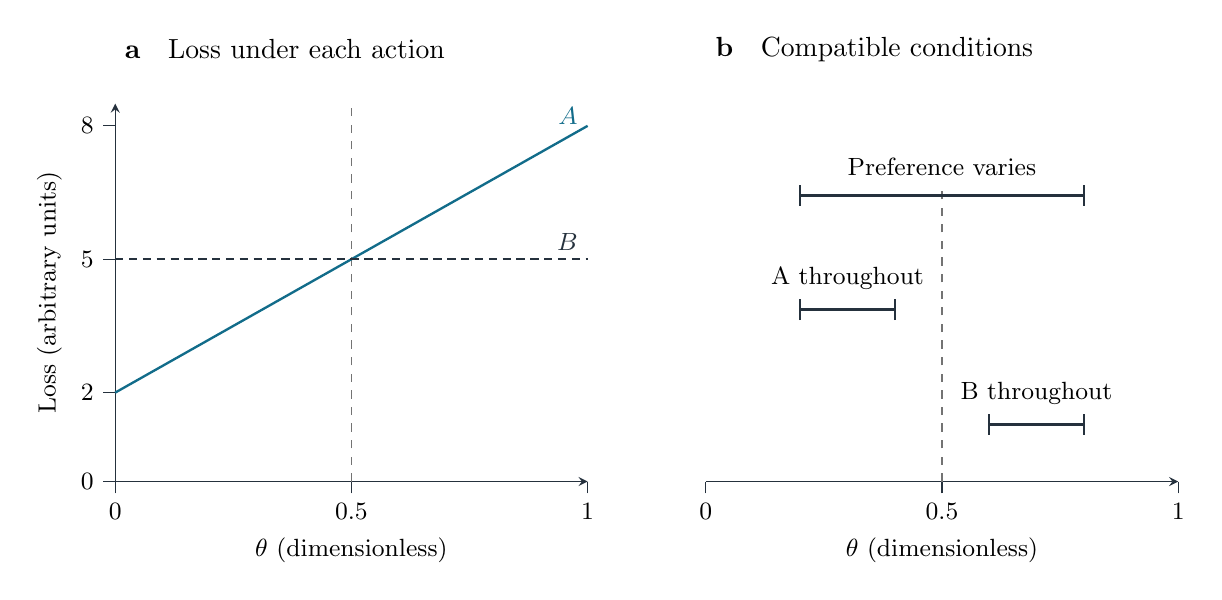
\begin{tikzpicture}[font=\fontsize{9}{11}\selectfont]
\definecolor{ink}{HTML}{25313D}
\definecolor{accent}{HTML}{126C8A}
\pgfplotsset{compat=1.18,
  decision axis/.style={
    width=60mm, height=48mm, scale only axis,
    xmin=0, xmax=1, xtick={0,0.5,1},
    axis lines=left, axis line style={line width=0.45pt, draw=ink},
    tick style={line width=0.45pt, draw=ink},
    tick align=outside, ticklabel style={font=\fontsize{9}{11}\selectfont},
    xlabel={$\theta$ (dimensionless)},
    xlabel style={font=\fontsize{9}{11}\selectfont},
    every axis plot/.append style={no marks},
    clip=false, enlargelimits=false}}
\begin{axis}[decision axis, name=losses, at={(0mm,0mm)}, anchor=south west,
  ymin=0, ymax=8.5, ytick={0,2,5,8},
  ylabel={Loss (arbitrary units)},
  ylabel style={font=\fontsize{9}{11}\selectfont},
  title={\textbf{a}\quad Loss under each action},
  title style={font=\fontsize{10}{12}\selectfont, at={(0,1.10)}, anchor=west}]
\addplot[draw=black!55, dashed, line width=0.45pt] coordinates {(0.5,0) (0.5,8.5)};
\addplot[draw=accent, line width=0.85pt] coordinates {(0.0,2.0) (1.0,8.0)};
\addplot[draw=ink, densely dashed, line width=0.85pt] coordinates {(0.0,5.0) (1.0,5.0)};
\node[anchor=south east, text=accent, inner sep=0pt] at (axis cs:0.98,8.02) {$A$};
\node[anchor=south east, text=ink, inner sep=0pt] at (axis cs:0.98,5.18) {$B$};
\end{axis}
\begin{axis}[decision axis, at={(75mm,0mm)}, anchor=south west,
  ymin=0.5, ymax=3.8, ytick=\empty, axis y line=none,
  title={\textbf{b}\quad Compatible conditions},
  title style={font=\fontsize{10}{12}\selectfont, at={(0,1.10)}, anchor=west}]
\addplot[draw=black!55, dashed, line width=0.45pt] coordinates {(0.5,0.5) (0.5,3.1)};
\addplot[draw=ink, line width=1.1pt] coordinates {(0.2,3) (0.8,3)};
\addplot[draw=ink, line width=0.6pt] coordinates {(0.2,2.91) (0.2,3.09)};
\addplot[draw=ink, line width=0.6pt] coordinates {(0.8,2.91) (0.8,3.09)};
\node[anchor=south, inner sep=0pt] at (axis cs:0.5,3.17) {Preference varies};
\addplot[draw=ink, line width=1.1pt] coordinates {(0.2,2) (0.4,2)};
\addplot[draw=ink, line width=0.6pt] coordinates {(0.2,1.91) (0.2,2.09)};
\addplot[draw=ink, line width=0.6pt] coordinates {(0.4,1.91) (0.4,2.09)};
\node[anchor=south, inner sep=0pt] at (axis cs:0.3,2.17) {A throughout};
\addplot[draw=ink, line width=1.1pt] coordinates {(0.6,1) (0.8,1)};
\addplot[draw=ink, line width=0.6pt] coordinates {(0.6,0.91) (0.6,1.09)};
\addplot[draw=ink, line width=0.6pt] coordinates {(0.8,0.91) (0.8,1.09)};
\node[anchor=south, inner sep=0pt] at (axis cs:0.7,1.17) {B throughout};
\end{axis}
\end{tikzpicture}

\caption[Evidence sufficiency for a bounded choice]{Illustrative evidence sufficiency.
\textbf{(a)} The actions have equal loss at $\theta=0.5$.
\textbf{(b)} Alternative compatible ranges either contain a preference reversal
or favour one action throughout. These hypothetical ranges are neither a sequence
nor confidence intervals. Stable preference supports stopping inquiry about this
uncertainty under the assumed model and remaining decision requirements.
Other decision rules can choose when preference varies. No globally minimal
evidence set is established.
}
\label{fig:decision-sufficiency}
\end{figure}

Proportionate argumentation also has a longer engineering history. HSE's 2006 offshore guidance calls for reasoned, supported arguments and assessment proportionate to the risk. It explains that even very high risks can call for qualitative assessment when the need for reduction is already obvious.\cite{hse} This illustrates why evidence effort should depend on what remains uncertain about the decision. Establishing a reason to stop an evidently unacceptable operation can require less analysis than establishing a reason to continue it.

This proportionality has direct backing. NIST's AI RMF 1.0 states that eliminating all negative risk can waste resources and that priorities and thoroughness should reflect assessed risk and impact.\cite{airmf} DORA reports an association between heavyweight external change approvals and poorer delivery performance, without evidence of lower change-failure rates. Its software-delivery findings favour capable peer review and automation; their observational basis does not establish that removing every approval improves every system.\cite{dora} NIST's agent-identity guidance also warns against overusing human approvals while advocating established identity and access controls.\cite{identity} These sources support selecting effective controls, rather than treating more oversight as a reliable proxy for better engineering.

Over-governance means imposing additional process whose contribution to the decision, risk control or applicable obligation cannot be justified relative to its cost. Assurance remains useful where it produces or tests a necessary reason for confidence. Repeated approvals that add neither independent scrutiny nor new decision-relevant information have no established assurance benefit here. An independent inspection of a disputed failure mechanism can be indispensable. Engineers should be able to explain both why an evidence request is necessary and why an additional request would be redundant. Applicable obligations constrain that judgement; they cannot be waived simply by calling them overhead.

The extended Toulmin reconstruction below makes the two claims and their support explicit. It retains Toulmin's claim, grounds, warrant, backing, qualifier and rebuttal, then adds the engineering context and action records described afterwards.\cite{toulmin} This is an operational engineering extension, rather than a claim that one universally standardised extended Toulmin model exists.

\begin{table}[htbp]
\small
\centering
\caption[Toulmin reconstruction of the two claims]{The connected arguments for explicit justification and proportionate inquiry.}\label{tab:toulmin}
\begin{tabular}{@{}
  >{\raggedright\arraybackslash}p{(\columnwidth - 4\tabcolsep) * \real{0.15}}
  >{\raggedright\arraybackslash}p{(\columnwidth - 4\tabcolsep) * \real{0.425}}
  >{\raggedright\arraybackslash}p{(\columnwidth - 4\tabcolsep) * \real{0.425}}@{}}
\toprule\noalign{}
\begin{minipage}[b]{\linewidth}\raggedright
Toulmin component
\end{minipage} & \begin{minipage}[b]{\linewidth}\raggedright
Claim A: explicit justification
\end{minipage} & \begin{minipage}[b]{\linewidth}\raggedright
Claim B: proportionate inquiry
\end{minipage} \\[4pt]
\midrule\noalign{}
\textbf{Claim} & Consequential AI delegation requires an inspectable justification for accepting the result and its intended use. & Engineers should obtain the minimum sufficient evidence for the decision and remove additional process lacking a justified contribution. \\[4pt]
\textbf{Grounds} & Historical assurance practice already connects evidence to claims; AI studies show task-dependent performance, misplaced confidence and failures at tool trust boundaries.\cite{sei,perry,sandoval,agentdojo} & Inquiry and approvals consume resources; NIST recommends risk-proportionate effort, and DORA finds no demonstrated stability advantage from heavyweight external approvals.\cite{airmf,dora} \\[4pt]
\textbf{Warrant} & Evidence supports a consequential use only through an applicable inference; exposing its assumptions allows others to challenge reliance. This is the normative engineering premise of the argument. & Additional work is justified by the uncertainty it resolves, the control it supplies or the obligation it fulfils, relative to its cost and delay. This is a decision principle, not an empirical law. \\[4pt]
\textbf{Backing} & Established assurance cases provide the evidence-to-claim structure; research on defeaters supplies a way to challenge it.\cite{standard,defeaters} & Risk-proportionate management and streamlined review support tailoring effort to the particular decision.\cite{airmf,dora} \\[4pt]
\textbf{Qualifier} & Applies where delegated work has material consequences and acceptance depends on uncertain or contestable inference. Existing adequate justification can be reused. & Applies after preserving material contrary evidence, required controls and applicable obligations. Sufficiency depends on consequence, reversibility and uncertainty. \\[4pt]
\textbf{Rebuttal and disposition} & Existing engineering arguments defeat the claim of historical novelty. Successful AI deployments defeat blanket pessimism. Neither removes the need to justify the particular use. & Serious unresolved failure conditions defeat a proposal to stop inquiry. Redundant approval and evidence gathering defeat a proposal to expand process merely because AI is involved. \\[4pt]
\bottomrule
\end{tabular}
\end{table}

For engineering use, attach the \textbf{context and assumptions} to each consequential inference: identify the decision owner, exact artefact or configuration, intended environment, operating interval and acceptance criterion. State open assumptions as conditions of the conclusion. An engineer should be able to see which assumption would change the decision if it failed. Evidence needs an origin, acquisition method and time, with uncertainty and known dependence recorded where relevant. Reusing one observation in several arguments creates no new corroboration. These additions make the Toulmin relations applicable to an identified engineering situation.

Record \textbf{challenge and disposition} at the point challenged. An underminer questions a ground, such as an unreliable measurement. An undercutter questions the inference, such as transferring an idle-system test to peak load. A rebutter supports an incompatible conclusion, such as an observed violation of the claimed limit. State whether the challenge is answered, changes the claim, defeats it or remains unresolved. Agreement between reviewers supplies no replacement for the evidence needed to resolve an empirical dispute. Failed support leaves a claim unestablished; asserting its negation requires its own grounds.

Connect the supported claims to \textbf{alternatives, decision and action} through a separate practical argument. The record should explain why the selected option is acceptable given consequences, uncertainty, constraints and the cost of delay. Include inaction or a smaller intervention when feasible. Record the authorised scope and action preconditions separately from claim support. An engineer may reasonably choose a controlled trial while a broader deployment claim remains unestablished. Authorisation permits an action; it does not establish the truth of a technical proposition. Retain the evidence available at decision time and distinguish it from later observations of execution and outcome.

Finally, define \textbf{reconsideration and inquiry stopping}. Name the change or observation that would require reassessment, and identify who or what will detect it. Reuse applicable evidence; refresh only evidence whose identity, scope or freshness no longer supports its role. Monitoring contributes only when the relevant condition is observable in time and an effective response exists. A nominal rollback is inadequate if the harm is irreversible. A successful outcome can inform future decisions without retroactively repairing an unsupported earlier inference.

Consider an illustrative service change, with no measured results implied. An agent proposes increasing a worker pool to reduce a queue. The engineer's immediate decision is whether to run a bounded staging trial. The relevant claim is that this trial has an acceptable effect on the isolated environment under the agreed resource cap. Required grounds might be the configuration diff, verified isolation and permission limits, and a check that the cap and stop mechanism work. A complete production-capacity case would answer a different question. The engineer can justify the trial without pretending to have established production readiness.

Suppose the trial then records lower queue delay. A decision to deploy needs a further inference: that the result applies under the proposed production conditions and that the increase does not cause an unacceptable competing effect. If database contention is the identified uncertainty that could reverse the choice, collect evidence about that contention under a relevant workload. Repeating unrelated unit tests or obtaining several signatures on the same latency chart will not resolve it. Conversely, credible evidence of resource exhaustion must remain in the argument even if delay improved. The decision follows the combined evidence and constraints.

A bounded rollout may require less prior evidence than an unrestricted release when limited exposure, timely detection and effective reversal make the remaining uncertainty acceptable. Those conditions require support. If the change can corrupt shared persistent data before detection, rollback may offer no adequate protection, and stronger prior evidence or a different action is required. The minimum sufficient evidence therefore changes with the action selected. Thinking through the alternatives can reduce evidence needs by changing the intervention itself.

For repeated cases, retain the justified decision rule and its applicability conditions. Automate checks for routine cases within that scope, and direct engineering attention to meaningful deviations. An approval is useful when the approver can supply missing competence, authority or a substantive challenge. Requiring a person to reconfirm an unchanged, already justified rule at every invocation needs separate justification. This is how the two claims work together: explicit reasoning identifies both the evidence that must be obtained and the work that can be omitted.

EAL/3 implements parts of this approach. Its \href{https://github.com/emmett08/earl/blob/main/docs/argument-model.md}{argument model} maps the six Toulmin functions to claims, evidence and premises, reasoning methods and backing, scope and targeted objections. Evidence declarations specify acquisition requirements; \href{https://github.com/emmett08/earl/blob/main/docs/argument-service.md}{observations and assessments} are retained separately. \href{https://github.com/emmett08/earl/blob/main/docs/argument-reconstruction.md}{Argument reconstruction} explains how to distinguish recovery of implicit reasoning from a proposed repair. These facilities can preserve the reasons relevant to a later assessment without requiring the model to reconstruct them from conversation alone.

The implemented limits constrain the claim for EAL. \texttt{structured/1} checks declared dependencies without proving that the authored rationale is sufficient; assessed prose remains \texttt{prose\_verified:\ false}. A \texttt{supported} result concerns the represented argument and observations, and supplies no release authorisation. Digests identify recorded content without establishing the authenticity of an untrusted producer. The registered workflow reassesses when requested and reuses compatible fresh observations; it is not an autonomous monitor of every relevant external change. Action enforcement, decision authority and detection of omitted physical conditions remain responsibilities of the surrounding engineering system.

EAL's acquisition planning also follows the authored routes, including declared challenges. It does not optimise a global minimum evidence set or discover every decision-relevant premise. The engineer must select the bounded question and justify its evidence requirements. Smaller packets, fewer calls or a successful interpreter are insufficient evidence of better decisions.

The repository's \href{https://github.com/emmett08/earl/blob/main/paper/README.md}{retained pilot and controlled follow-up} provide narrower measurements. The diagnostic follow-up reports whole-verdict reference agreement with internal consistency in 30 of 40 EAL recipient answers and 33 of 40 conventional-evaluator answers, with byte-identical EAL and conventional model-visible packets in all 40 pairs. It therefore cannot identify an EAL notation advantage. Its authored cases, limited execution and AI coding restrict inference. A wider benefit claim would require comparable evidence access and decision rules, independently assessed outcomes, and measurement of acquisition, review, delay and incident costs. The argument for inspectable justification does not depend on EAL winning that comparison.

The proposed shift is consequently precise: make the justification for consequential delegation a maintained part of engineering work, and let the decision determine the necessary inquiry. Begin with one consequential workflow. Identify the choice and the uncertainty that could change it; reuse applicable evidence; obtain the missing discriminating evidence; record the inference and strongest challenge; then act within the justified scope. Retain only the process needed to preserve that justification, enforce the action boundary and detect conditions requiring reconsideration.

\textbf{References and source scope.} Sources checked on 3 October 2026. Primary-source observations and recommendations are cited below; the two claims, their engineering extension and the illustrative service example are this document's synthesis. Publication or formal structure alone establishes neither content quality nor effectiveness.

\FloatBarrier
\begin{thebibliography}{99}
\small
\raggedright
\interlinepenalty=10000
\setlength{\parskip}{0pt}
\setlength{\itemsep}{4pt}
\bibitem{nasa}
NASA (2016), \emph{NASA Systems Engineering Handbook}, NASA/SP-2016-6105 Rev2. \href{https://www.nasa.gov/wp-content/uploads/2018/09/nasa_systems_engineering_handbook_0.pdf}{Official handbook}; \href{https://www.nasa.gov/reference/6-0-crosscutting-technical-management/}{chapter 6}. Locators: §§5.3--5.4 and §§6.2--6.8; \href{https://www.nasa.gov/reference/6-8-decision-analysis/}{§6.8.1} on further inquiry and §6.8.1.3.1 on the decision record.

\bibitem{sei}
Charles B. Weinstock and John B. Goodenough (2009), \emph{Towards an Assurance Case Practice for Medical Devices}, CMU/SEI-2009-TN-018. \href{https://sei.cmu.edu/library/towards-an-assurance-case-practice-for-medical-devices/}{Official report and abstract}, DOI: 10.1184/R1/6585389.v1. Historical evidence of explicit safety argumentation; the report illustrates an infusion-pump case.

\bibitem{standard}
ISO/IEC/IEEE 15026-2:2022, \emph{Systems and software engineering---Systems and software assurance---Part 2: Assurance case}. \href{https://standards.ieee.org/ieee/15026-2/10236/}{Official scope}; \href{https://standards.ieee.org/ieee/15026-2/5234/}{2011 predecessor}. The public scope specifies structure and meaning without prescribing content quality or a particular representation. No claim here depends on inspection of the paid standard's full text.

\bibitem{census}
Adam Grundy, Cory Breaux and Dhanapati Khatiwoda (2026), \href{https://www.census.gov/library/stories/2026/05/ai-use-businesses.html}{``Large Firms With at Least 20 Employees Biggest AI Users''}, US Census Bureau, 26 May. Locators: ``U.S. Business AI Use'' and ``AI Trends Across Sectors''; nationally representative BTOS, with a changed question from November 2025.

\bibitem{microsoft}
Microsoft (2025), \href{https://www.microsoft.com/en-us/worklab/work-trend-index/2025-the-year-the-frontier-firm-is-born}{``2025: The Year the Frontier Firm Is Born''}, Work Trend Index, 23 April. Locators: agent-workflow finding and ``Survey Methodology''; online fieldwork, February--March 2025. Deployment reports, future intentions and population prevalence are distinct quantities.

\bibitem{perry}
Neil Perry, Megha Srivastava, Deepak Kumar and Dan Boneh (2023), ``Do Users Write More Insecure Code with AI Assistants?'', \emph{ACM CCS}, pp.~2785--2799, DOI: 10.1145/3576915.3623157. \href{https://arxiv.org/abs/2211.03622}{Open paper}. Locators: abstract and study/results sections. The assistant used codex-davinci-002; the result is not an estimate for current models generally.

\bibitem{sandoval}
Gustavo Sandoval et al.~(2023), ``Lost at C: A User Study on the Security Implications of Large Language Model Code Assistants'', \emph{USENIX Security}, pp.~2205--2222. \href{https://www.usenix.org/conference/usenixsecurity23/presentation/sandoval}{Official paper and abstract}. A bounded counterexample to uniform claims of adverse security effects; the task was a linked shopping-list structure in C.

\bibitem{benefits}
Erik Brynjolfsson, Danielle Li and Lindsey Raymond (2025), ``Generative AI at Work'', \emph{Quarterly Journal of Economics}, 140(2), pp.~889--942, DOI: 10.1093/qje/qjae044. \href{https://arxiv.org/abs/2304.11771v2}{Open author version}, abstract and empirical analysis. A staggered workplace rollout; generalisation to autonomous engineering agents requires separate evidence.

\bibitem{agentdojo}
Edoardo Debenedetti et al.~(2024), ``AgentDojo: A Dynamic Environment to Evaluate Prompt Injection Attacks and Defenses for LLM Agents'', \emph{NeurIPS}, Datasets and Benchmarks Track. \href{https://arxiv.org/abs/2406.13352}{Open paper}, abstract and §§3--4. Evidence of benchmark failure mechanisms, not a population incident estimate.

\bibitem{genai}
Chloe Autio et al.~(2024), \emph{Artificial Intelligence Risk Management Framework: Generative Artificial Intelligence Profile}, NIST AI 600-1. \href{https://nvlpubs.nist.gov/nistpubs/ai/NIST.AI.600-1.pdf}{Official report}, DOI: 10.6028/NIST.AI.600-1. Locators: §§2.2 and 2.7; actions MS-2.5-001 and MS-2.5-003. Guidance and risk characterisation, rather than proof that argumentation reduces incidents.

\bibitem{defeaters}
Robin Bloomfield, Kate Netkachova and John Rushby (2024), \emph{Defeaters and Eliminative Argumentation in Assurance 2.0}, SRI-CSL-2024-01. \href{https://arxiv.org/abs/2405.15800}{Open report}. The abstract and technical account distinguish positive support from recorded challenges and their resolution; method backing, rather than an effectiveness trial.

\bibitem{hse}
Health and Safety Executive (2006), \emph{Guidance on risk assessment for offshore installations}, Offshore Information Sheet 3/2006. \href{https://www.hse.gov.uk/offshore/assets/docs/sheet32006.pdf}{Official guidance}, pp.~1--4. Historical offshore-specific guidance illustrating supported argument and proportionate assessment; the reference is not a statement of current legal requirements for other sectors.

\bibitem{airmf}
NIST (2023), \emph{Artificial Intelligence Risk Management Framework (AI RMF 1.0)}, NIST AI 100-1. \href{https://nvlpubs.nist.gov/nistpubs/ai/NIST.AI.100-1.pdf}{Official report}, DOI: 10.6028/NIST.AI.100-1. Locators: §§1.2.2--1.2.4, especially §1.2.3 on prioritisation. Supports proportionality and integration with existing risk management.

\bibitem{dora}
DORA, \href{https://dora.dev/capabilities/streamlining-change-approval/}{``Capabilities: Streamlining change approval''}. Locators: opening research findings and implementation guidance. Research-based software-delivery guidance; associations do not establish a universal causal effect of removing approvals.

\bibitem{identity}
Bill Fisher and Ryan Galluzzo (2026), \href{https://www.nist.gov/blogs/cybersecurity-insights/back-future-why-agentic-ai-needs-strong-identity-foundation}{``Back to the Future: Why Agentic AI Needs a Strong Identity Foundation''}, NIST, 27 August. Locators: authorisation, human-in-the-loop discussion and closing recommendations. Engineering guidance on established controls, not a measured argumentation benefit.

\bibitem{toulmin}
Stephen E. Toulmin (2003 {[}1958{]}), \emph{The Uses of Argument}, updated edition, Cambridge University Press, chapter III, pp.~87--134. \href{https://www.cambridge.org/core/books/abs/uses-of-argument/layout-of-arguments/0CF09834F2802518330E754858CC0655}{Publisher chapter and DOI}. Foundation for the six argument functions; the engineering additions above are explicitly separate.
\end{thebibliography}
\end{document}
